\documentclass[12pt, dvipsnames, a4paper]{article}
\usepackage{geometry}
\geometry{legalpaper, margin=0.5in}
\usepackage{xcolor}
\usepackage{xspace} 
\usepackage[normalem]{ulem}
\usepackage{vwcol}
\usepackage{cancel}
\usepackage{enumitem}
\usepackage{amsmath}
\usepackage{caption}
\usepackage{graphicx}
\usepackage{amsfonts}
\usepackage{float}
\usepackage{multicol}
\usepackage{hyperref}
\usepackage{listings}
\usepackage{textcomp}
\usepackage{lstautogobble}
\usepackage[parfill]{parskip}
\usepackage{tikz-qtree}
\usepackage{tikz}
\usepackage{hyperref}
\usetikzlibrary{decorations.pathreplacing}
\tikzset{every tree node/.style={minimum width=4cm,draw,circle},
         blank/.style={draw=none},
         edge from parent/.style=
         {draw,edge from parent path={(\tikzparentnode) -- (\tikzchildnode)}},
         level distance=1.5cm}

%% Genearl %%
\renewcommand{\thesection}{\arabic{section}}

%% For convenience %%
\newcommand{\code}[1]{\texttt{#1}}
\newcommand{\bcode}[1]{\texttt{\textbf{#1}}}
\newcommand{\balert}[1]{\textbf{\alert{#1}}}
\newcommand{\rarrow}{$\Rightarrow$}
\newcommand{\tab}[1][0.5cm]{\hspace*{#1}}
\newcommand{\deepemphasis}[1]{\underline{\textbf{\Large{#1}}}}
\newcommand{\bfemph}[1]{\textbf{\emph{#1}}}
\newcommand{\OR}[0]{\lvert \: \rvert}

%% Colours %%
\definecolor{mLightBrown}{HTML}{EB811B}
\definecolor{mLightGreen}{HTML}{14B03D}

%% Pseudocode %% 
\lstdefinelanguage{pseudo}
{
	keywords=[1]{
		class,
		new,
		loop,
		until,
		end,
		if,
		else,
		then,
		return,
		while,
		for,
		to,
		fun,
		break,
		and,
		true,
		false,
		or,
		do,
	},
	keywordstyle=[1]\color{black}\bf,
	keywords=[2] {
		invariant,
		precond,
		postcond
	},
	keywordstyle=[2]\color{blue}\bf
}

\lstset{
	language 		= 	pseudo,
	basicstyle		=	\ttfamily,
	mathescape		=	true,
	escapeinside	=	||,
	tabsize			=	2,
	numbers			=	left,
	commentstyle	=	\color{OliveGreen},
	stringstyle		=	\color{mLightBrown},
	upquote			=	true,
	morestring		=	[b]',
	moredelim		=	[l][\rmfamily\itshape]{@},
	comment			=	[l]{//},
	morecomment		=	[s]{/*}{*/},
	commentstyle=\color{Gray}\ttfamily,
	showstringspaces=	false,
	showtabs		=	false,
	autogobble
}

%% Other %%
\setcounter{secnumdepth}{5}
\setcounter{tocdepth}{5}


%**************************************************************************************************************%
%______________________________________________________________________________________________________________%

\begin{document}
\title{\textbf{EECS 3311 - Lab 05\\Design Report}}
\author{Amir Mohamad, Saniz Momin, Akif Prasla, Hasnain Saifee\\\\TA - ta name}
\date{Nov 7, 2021}
\maketitle
\tableofcontents
\clearpage

\section{Introduction}

The software project is about generating a soccer game where there are two players:
a goalkeeper and a striker. You have 60 seconds to score as many goals as possible,
after each goal is scored your score increments and the game is paused. You can resume
the game by pressing key R or by going to the menu option selecting control which has a
sub menu resume and pause. To score a goal the striker can move by pressing up down left
right key and to score a goal striker has to press space key. The goalkeeper randomly defends
the gate by moving in the left and right direction bounded by the gate's length. After the
timer becomes 0 the user gets the statistics of how many goals the striker has scored and how
many saves has the goalkeeper made. When the game is over, the user can start playing again
by navigating to the menu bar, clicking on the Game menu and clicking to a new game or exit
if the user wants to end playing. The main-goal of this software project is to use OOP concepts
and efficient software design patterns to write code efficiently and follow the DRY principle
which is (Don't repeat yourself). In this software project, to properly organize our soccer
game system, the system is divided into a set of layers where each layer focuses on a
specific aspect and has an abstraction level. MVC architectural pattern is used to divide
the system into three main subsystems where the model comprises data of the system, for
example keeping record of total goals and saves of striker and goalkeeper respectively.
The view consists of the user interface part where the data in the model subsystem can be
viewed. The controller which handles interaction between the modal and the view. The detailed
design of the software system can be seen using creational design patterns such as factory
design pattern as well as prototype design pattern which focuses on creation of objects.
For example players are created via the PlayerFactory class which has getplayer method
which takes string as parameter. All that is needed to pass is a string and it will
return the appropriate object. Doing a project with partial implementation takes time
to understand the logic and the functionality of code written. It took a while until
we all understood what is the role of each subsystem, once we got that it was easy to
implement and finish the rest. Based on our understanding of this software project we
are going to write the report with the basic idea and the designs implemented for the
top level and organization of the software project. We will create a UML diagram to make
our explanation of the design patterns used more clear. We will then explain the main
elements in this system and explain their functionalities. We will conclude our report
by giving brief overview of our journey in building this software project.

\section{System Design}
\subsection{Overview}
\begin{center}
	\begin{figure}[H]
		\hspace{50pt}
		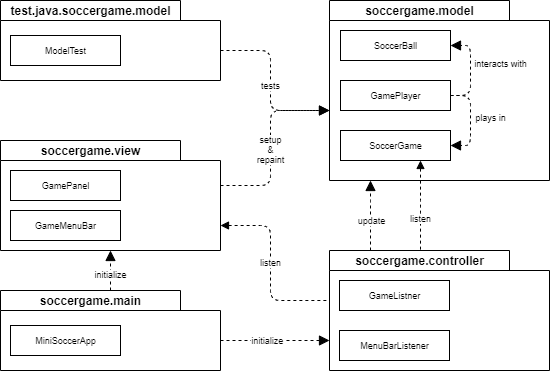
\includegraphics[scale=0.6]{diagrams/system-diagram/system-diagram-pkg.png}
		\caption{The system design \code{SOCCERGAME}'s (example placeholder image)}
		\label{fig:systemdeisgn}
	\end{figure}
\end{center}
\clearpage

\section{Front end}
\subsection{Overview}
short description overview of front end
\subsection{Class Diagram}
\begin{center}
	\begin{figure}[H]
		\hspace{50pt}
		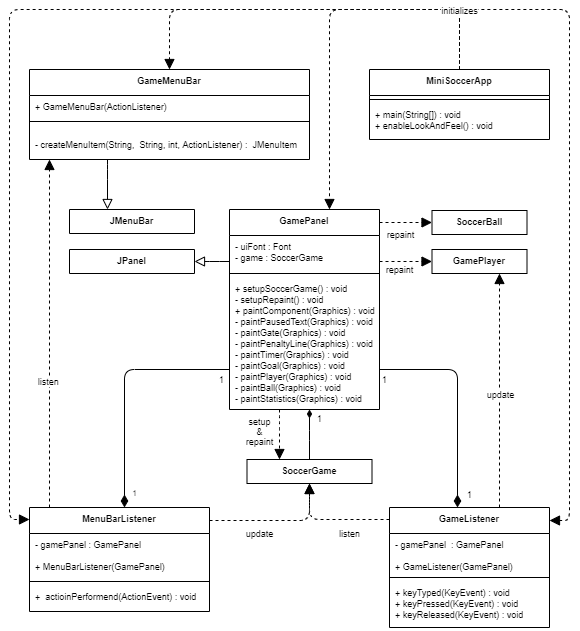
\includegraphics[scale=0.6]{diagrams/class-diagrams/gui-model/gui-model-cd.png}
		\caption{The class diagram of \code{SOCCERGAME}'s front end model (example placeholder image)}
		\label{fig:frontend}
	\end{figure}
\end{center}
\clearpage

\section{Classes}
\subsection{MiniSoccerApp}
The main runner class which runs the whole project.
\subsection{GameMenuBar}
This class represents the top portion of the view which has various controls such as resume, new game, end game, exit,etc
\subsection{GamePanel}
This class initiates the main view and gives user a visual representation of the game inside the frame. All the visual components
such as frame, color, etc. are contained in this.
\subsection{GameListener}
This is a control class which connects the model and view. This controls the user action such as movement and goal scored by connecting
the other two packages.
\subsection{MenuBarListener}
This is a control class which connects model and view. this class gives the functionality of resume and paused buttons so when
paused button is pressed the whole game is paused along with the timer and when resume button is pressed game resumes. there is also
a new Game button which loads and starts the game again.
\clearpage

\section{Back end}
\subsection{Overview}
In this software project we are using combination of factory design pattern and prototype design pattern.
we have used combination of both in such a way that we are fulfilling the goal of factory design by hiding the
creation of object. prototype design pattern is used here keeping performance in mind i.e. other players such as
GoalKeeper and Striker doesnt have code repitition since they extend an abstract GamePlayer class which contains
necessary common methods thus reducing code repitition and keeping up the DRY rule which is (Dont repeat yourslef).

\subsection{Class Diagram}
\begin{center}
	\begin{figure}[H]
		\hspace{30pt}
		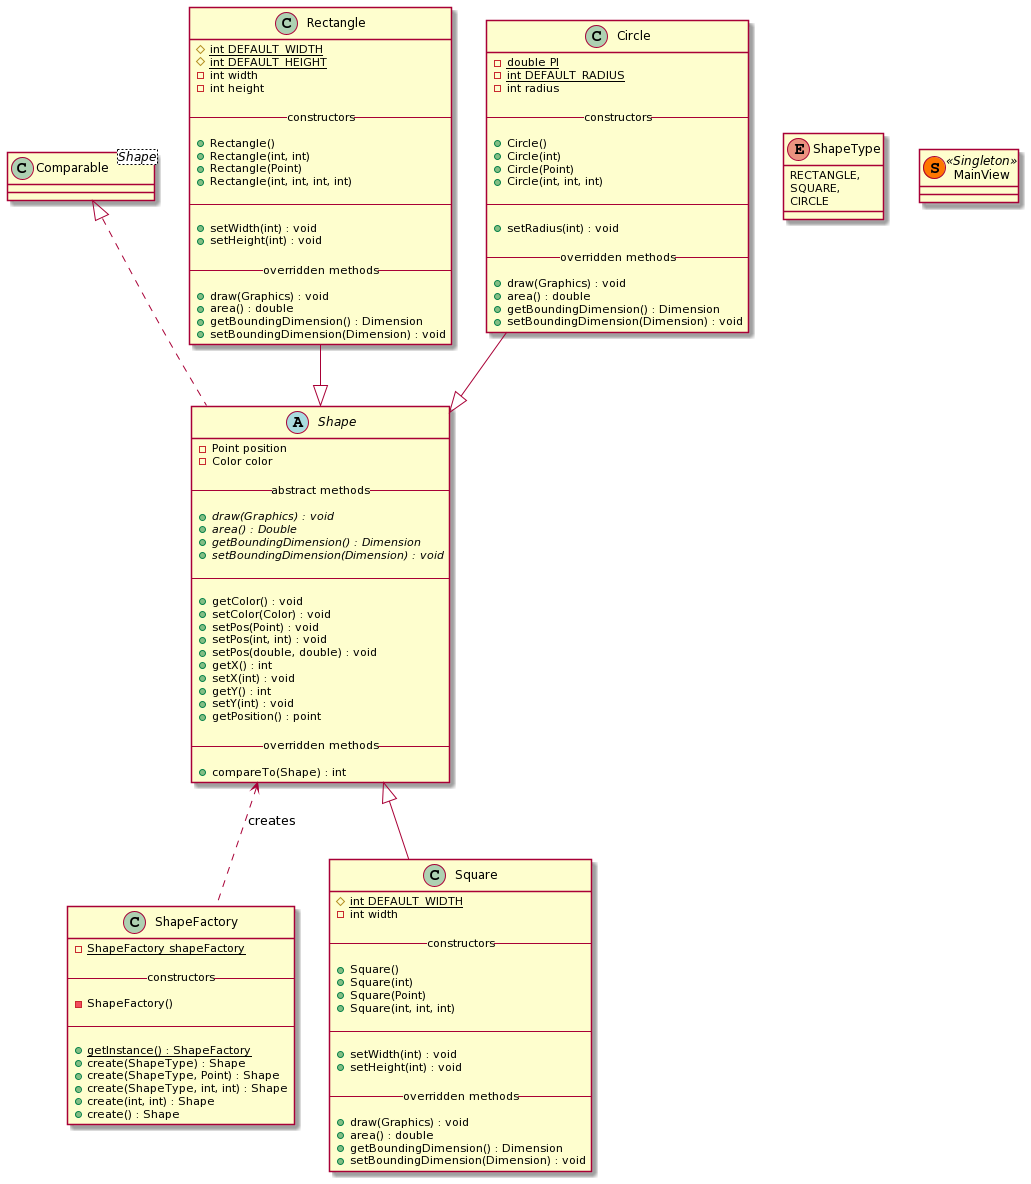
\includegraphics[scale=.5]{diagrams/class-diagrams/shape-model/shape-model-alt-cd.png}
		\caption{The class diagram of \code{SOCCERGAME}'s player model (example placeholder image)}
		\label{fig:backend}
	\end{figure}
\end{center}
\clearpage

\section{Classes}
\subsection{GamePlayer}
This is one of the important class required in this software project it is an abstract class
and contains  essential methods such as moveLeft, moveRight, moveUp,moveDown, shootBall. without the GamePlayer
class there is no existence of two players the goalKeeper and striker without which the soccerApp has no meaning.
\subsection{GoalKeeper}
This is the class which fulfills the role of goalKeeper. it keeps record of number of saves through
playerStatistics class. it has functionality of moving randomly left-right guarding the goalpost.
\subsection{Striker}
This is the class which fulfills the role of a striker. the purpose of moving near to the goalpost
and scoring goals is what this class does with the help of methods inherited from its parent GamePlayer such as
movingUP down left right and shooting the ball.
\subsection{PlayerStatistics}
This class contains the statistics such as score.
\subsection{PlayerCollection}
\subsection{PlayerCollectionIterator}
This class works as an iterator class and helps other classes which need to iterate.
\subsection{PlayerFactory}
\subsection{SoccerGame}
This class contains all the important aspects as it has the object notations of the other classes like PlayerCollection and it then
calls the PlayerFactory class to further initiate the GamePlayer(goalkeeper and striker).
\subsection{SoccerBall}
This class represents the ball of the game and deals with the positioning of the ball when in play.

\clearpage

\subsection{OOP Principles}
\textbf{Abstraction}: In this software project, some unnecessary details are hidden from other classes. We will give you examples
where abstraction is used. Take a look at the PlayerFactory class which is used to generate players such as goalkeeper
and striker. The way object is created is completely hidden, what is done is a string is passed such as "goalkeeper" or
"striker" and object is returned.

\textbf{Encapsulation}: In this software project, you will see the concept of encapsulation used where some logical implementation
required for some classes to give required functionality is set to private so that other classes cannot access it.
Examples such as GamePanel class has private paint methods such as paintPausedText(), paintGate(), paintPentaltyLine() etc
as they are only required for the proper implementattion of the GamePanel class.

\textbf{Inheritance}: The concept of Inheritance is one of the most required principle used in this software project for better performance reasons.
The GamePlayer class which is the parent class of goalKeeper and striker, doing this has enabled us to reduce code repititoin significantly.
No child class even needed their own fields all they have is methods implemented which they inherited from GamePlayer class.

\textbf{Polymorphism}: In this software project the concept of polymorphism is also used. You will see in the PlayerFactory class that
players are instantiated with the syntax GamePlayer goalKeeper = PlayerFactory.getPlayer(“goalkeeper”) which upon decoding means Goalkeeper goalkeeper = new GoalKeeper();
Polymorphism means “many forms” therefore though the object created is of the GamePlayer class but the methods takes form according to the
new SpecificPlayer() where (SpecificPlayer- goalkeeper, striker) and whenever any method is invoked such as striker.shootBall()it uses the implementation
of that specificPlayer class though the instant type is GamePlayer this happens because of inheritance where it is considering the latest form of the method.
Therefore if it is GamePlayer goalkeeper =  new GoalKeeper() and if goakKeeper.shootBall() is invoked this will call the
latest implementation of shootBall() which is implemented in the GoalKeeper class.

\subsection{Design Patterns}
\textbf{Singleton}: \\
\textbf{Iterator}: \\
\textbf{Factory}:
\clearpage

\section{Implementation}
\subsection{Class Implementation}
This projects after reading all the requirements and design steps was initializing a java
gradle project using \code{gradle init} task, then customizig it to fit our project. After this, we started implementing
the required classes in IntelliJ or Eclipse. Since our team used git we were able to work on different development environment.
The IDEs in combination with gradle helped us compile and run our project. After the inital setup was completed, we iteratively
started working on the classes while testing them. The key members in testing our project so we improved our
coverage were Saniz, Akif and Hasnain. Using gradle helped to manage \code{jacoco} and \code{junit} dependencies so we can use
the TDD (Test driven development). We compiled our java classes with java 16 with the help of our IDEs and the \code{gradle run} command.
In this project, gradle is used it to manage the look and feel dependencies, create a \code{jacoco} coverage report, and provide an easy
way to run the project. Git was used along with Github so our team could collaborate effectively (this came in handy since we were all in different
time zones).

\subsection{Collection}
\subsection{Sorting}
\subsection{JavaDoc}
\subsection{JaCoCo}



\subsection{Execution}
disscuss execution process using gradle
\section{Tools}
\subsection{Source Code}
\textbf{IDE}: IntelliJ IDEA 2021.2.1 and Eclipse, to implement Java classes\\
\textbf{Documentation}: vscode, \LaTeX, for documentation (dessign report, etc.)
\subsection{Build}
\textbf{Build}: Gradle 7.2 (to manage dependencies and build)\\
\textbf{Java Version}: openjdk version "16.0.1" 2021-04-20\\
\textbf{Version Control}: Git with Github \\
\textbf{Unit Testing}: junit-jupiter-engine:5.8.1\\
\textbf{Coverage}: JaCoCo library, Codcov\\
\textbf{Github Actions}: used to neatly assert validity of tests before pull requests and pushes to main
\clearpage

\section{Conclusion}
This software project helped us to work as a group and also get an insight of how to collaborate while working on the same project.
We learned how to work in team and coordinate with each other. This project also helps us understand the design principles and use
them in an adequate way according to the project need. One bad thing was that we tried to work on the whole project at once and finish
it up quickly. This turned out to be a bad idea. We stepped back a little and went through the code bit by bit and understood how the
code is connected and what’s missing. We also traced the code on a paper which helped us a lot. The things that I learned through the
journey of creating this software project is initial planning, if it’s a project which requires lot of demand to be fulfilled. I used
divide and rule principle where I breakdown the demands of this project into subpart and tried to find what should be the role of that
subpart in the project how many classes will be required and is there a way to implement code reusability by using OOP Principles. We also
learned how to work thoroughly with github and collaborate when working on the same project. We learned design principles which were taught
to us and how to implement them in our project. Another thing we learned is how to manage time efficiently as we were all in different time zones.
The advantages of working as a group is that we get to learn concepts from various perspectives. This opens the way to go forward and choose the
most efficient path to reach the final output. Disadvantages can be difficult to find a common time for collaborating, too many ideas to deal with, etc.
Few recommendations for easy completion of project for upcoming students are that they should ask for help understanding the flow of code
in the project, attend lab session and ask for help from TA, make sure that they understand the basic concepts of JAVA and also the software
concepts taught in the class.

\subsection{Roles}
\textbf{Setup}: Amir\\
\textbf{Testing}: Amir, Saniz\\
\textbf{Uml}: Akif, Hasnanin\\
\textbf{Report}: Saniz, Akif, Hasnain\\

\end{document}
